%----------------------------------------------------------------------------
\chapter{Meta learning}
%----------------------------------------------------------------------------

Ebben a fejezetben ismertetem a metatanítás fogalmát, a megközelítéseket. Megmutatom, hogy mit old meg a few-shot learning és ez hogyan felhasználható nyílt halmazú beszélőfelismerő rendszerekben.
	 

\begin{displayquote}
	''--- Miért van szüksége a neurális hálózatoknak sok tanítómintára a jó teljesítéshez? Egy két éves gyerek miután látott pár autót képes felismerni azt.
	--- Egy ekkora gyereknek volt két éve tapasztalatokat szerezni olyan dolgokról, amik nem autók voltak. Biztos vagyok benne, hogy ez fontos szerepet játszott a dologban.''\newline
	\null\hfill (Quora)
\end{displayquote}

Az emberek képesek hasznosítani a korábban szerzett tudást. Ha valaki megtanult biciklizni, utána sokkal
könnyebben motorbiciklire ül. Felismerünk dolgokat úgy, hogy előtte csak néhányszor láttuk élőben vagy csak képen láttuk.

Az emberekkel szemben a neurális hálózatokkal két probléma van.

\begin{enumerate}
	\item Nem tanulnak effektíven, sok tanítómintát igényelnek
	egy feladat megtanulásához.  
	\item Nem hasznosítják a korábban, más feladatok által megszerzett tudást.
\end{enumerate}



Metatanítás alatt olyan tanító módszerek
összességét értjük, amelyek felhasználják a korábban szerzett tudást és hasznosítják azt a későbbi
feladatok során. A metatanuló modellek általánosítják a tapasztalataikat és könnyen adaptálódnak új
feladatokhoz. A könnyű adaptáció alatt kevés tanítómintával végzett tanítást értünk, más néven finomhangolást.


\section{Few-shot learning}

A neurális hálózatok rengeteg
tanítómintát igényelnek. A kevés tanítómintával
tanított hálózatok túltanulnak; a tanítóhalmazon jó eredményt mutatnak, de csökken az általánosító képességük, így a teszthalmazon jelentősen rosszabb eredményt érnek el. Ugyanakkor ha sok tanítómintával tanítjuk a hálózatokat, az adott feladatokra már jól általánosítanak, de magukra a feladatokra tanítjuk túl őket. További hasonló feladatokra nem tudnak általánosítani.

A few-shot learning azzal a problémával foglalkozik, hogy hogyan építhetünk olyan modelleket, amelyek képesek új feladatokat gyorsan megtanulni. A
modellt sokféle feladatra tanítjuk, de minden feladathoz kevés tanítóminta tartozik. A tanítás után új feladat esetén a modell kevés tanítómintával képes jól megtanulni azt. 

A few-shot learningre való képességet az n-way k-shot feladattal szokták mérni. 

\begin{enumerate}
	\item A modell kap egy eddig nem látott osztályból egy tesztmintát.
	\item Kap továbbá egy ún. segéd adathalmazt, ami az összes k eddig nem látott osztályból n mintát tartalmaz.
	\item Az algoritmus el kell döntse, hogy melyik osztályba tartozik a tesztminta a segédhalmazból.
\end{enumerate}

A beszélőfelismerő rendszereket tekintve nagyon fontos, hogy a neurális hálózat rugalmas legyen a tanulás szempontjából. Tegyük fel, hogy egy cég telefonos, szövegfüggetlen,
nyílt halmazú beszélőfelismerést szeretne abból a célból, hogy a betelefonáló kliensek adatait rövid hangminta után a rendszer automatikusan kilistázza az operátornak.
Egy nagyobb telefontársaság esetén ez több ezer beszélőt is jelenthet. Hagyományos neurális hálózatokkal minden egyes klienstől több perces hangmintára lenne szükség,
hogy ne tanítsuk túl a modellt. 

A másik, még nagyobb probléma, hogy új, vagy távozó kliens esetén újra kell tanítani a teljes hálózatot. A few-shot learning tökéletesen
megoldja mindkét problémát. Kevés tanítómintával -- regisztrációkor pár kérdés kliensenként -- működik a rendszer és rugalmas is tanítás szempontjából; új kliens esetén
hozzáadjuk a segédhalmazhoz a hangmintáját, távozáskor pedig eltávolítjuk.

\section{Metrikus metatanítás}

Metrikus metatanítás során a modell a tanítóminták halmazán egy távolságfüggvényt tanul meg.

\begin{equation} \label{eq:3}
P_{\theta}(y|x, S) = \sum_{(x_i, y_i)\in S} k_{\theta}(x, x_i)y_i
\end{equation}

A valószínűsége annak, hogy a $\theta$ modellparaméterekkel az $x$ minta $S$ segédhalmaz mellett az $y$ osztályba tartozik egyenlő a segédhalmazba tartozó címkék súlyozott összegével. A súlyt a $k_{\theta}$ ún. kernel függvény számolja ki. A kernel függvény az a távolságfüggvény, amit a modell megtanul.

A megközelítésre több implementáció is létezik, mint például a Matching Network, Prototypical Network, Relation Network és a konvolúciós sziámi hálózat. Ezek közül az utolsót fogom részletesen bemutatni.  

\subsection{Konvolúciós sziámi hálózatok}

A konvolúciós sziámi hálózatok két konvolúciós ikerhálózatból épülnek fel, amelyek megosztott súlyokat és rétegeket használnak. A hálózat két bementet kap, és miután a konvolúciós rétegek kiszámolták a jellemző vektorokat, ezeknek egy $\k_{\theta}$ távolságfüggvénnyel méri a hasonlóságát. Ha a hasonlósági pont meghalad egy küszöbértéket, a két képet hasonlónak tekintjük, egyébként különbözőnek.

\begin{figure}[!ht]
	\centering
	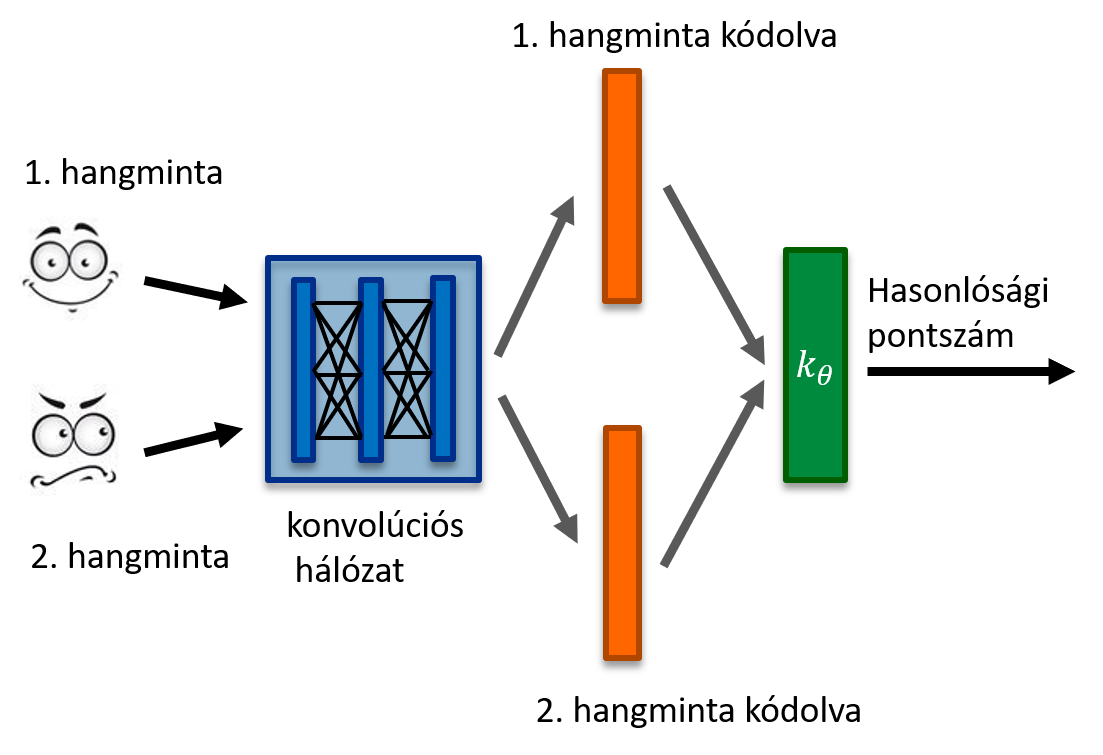
\includegraphics[width=100mm, keepaspectratio]{figures/siamese-cnn-arch.png}
	\caption{Konvolúciós sziámi hálózat architektúrája.}
	\label{fig:siamese-cnn-arch}
\end{figure}

Sok ábrán a sziámi hálózatokat két azonos hálózattal reprezentálják. Valójában mivel a két ikerhálózat súlyai és rétegei megosztottak, elég egy hálózatot használni és csak a jellemző vektorokat eltárolni, így kevesebb erőforrást használunk.

Működésük közben egy mintáról nem azt tanulják meg, hogy melyik osztályba tartozik, hanem a különbséget a többi mintához képest. Tanítás közben a konvolúciós hálózatot súlyait javítják, hogy az általa képzett kódolások azonos minták esetén azonosak, különbözők esetén pedig különbözőek legyenek, így a távolságfüggvény jól fog működni.

A konvolúciós sziámi hálózatok megoldást jelentenek a few-shot learning problémára, mert kevés tanítómintával is jól működnek. Vegyük példaként egy vállalat arcfelismerő rendszerét. A sziámi hálózatnak elég egy segédhalmazban egy-egy képet eltárolni minden alkalmazottról. Amikor egy alkalmazott a rendszert használja, a képét összehasonlítja a segédhalmazban lévő képekkel és a hasonlóság alapján dönt. Ezzel két problémát old meg:

\begin{enumerate}
	\item Egyrészt nem szükséges minden alkalmazottról több képet készíteni.
	\item Másrészt új alkalmazottak érkezése, vagy egy alkalmazott távozása után nem szükséges újra tanítani a hálózatot.
\end{enumerate}

A sziámi hálózatoknak a legismertebb költségfüggvénye a \emph{triplet loss} függvény. Ezt a \emph{gradient descent} módszerrel optimizálva tanítjuk a hálózatot. A triplet loss három bemenetet igényel, amelyek jelen példában a képekből képzett jellemző vektorok. Az egyik egy rögzített kép vektora, ez az ún. \emph{anchor}. A másik kettő pedig egy pozitív és egy negatív minta. Az egyik ugyanabból az osztályból származik mint az \emph{anchor} kép, a másik különbözőből.
\begin{equation}\label{eq:4}
	\mathcal{L}_{triplet}(A, P, N) = \max(d(A, P) - d(A, N) + m, 0)
\end{equation}

A $d$ a távolságfüggvény, ami lehet például euklideszi távolság. A \emph{triplet loss} veszi az anchor és a pozitív meg az anchor és a negatív minta távolságainak különbségét, majd ezt eltolja az $m$ küszöbértékkel. Ha az előbbi pozitív ezt veszi eredményül, egyébként nullát.

\begin{figure}[!ht]
	\centering
	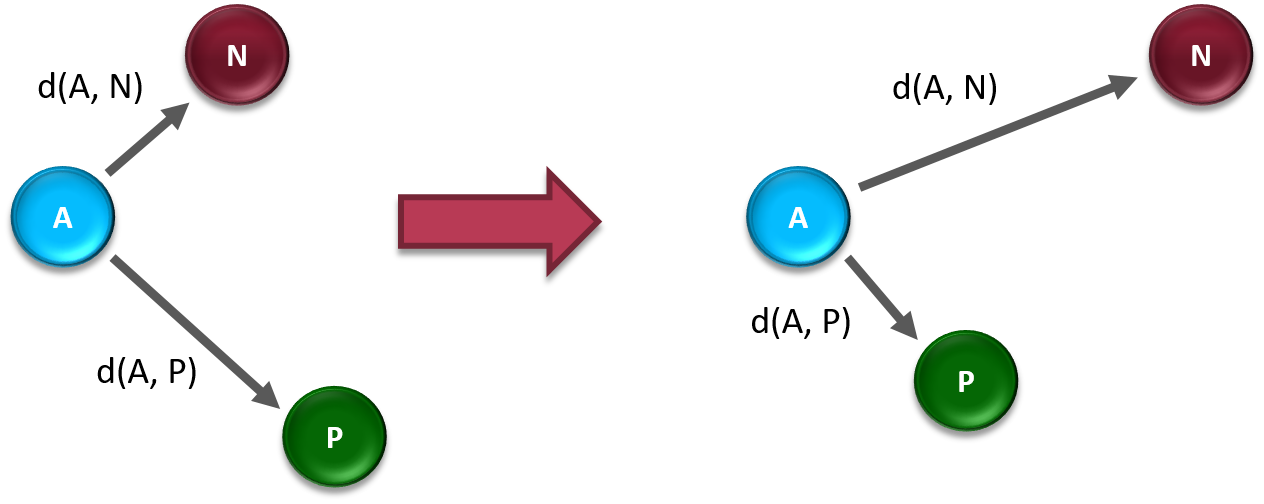
\includegraphics[width=100mm, keepaspectratio]{figures/triplet-loss.png}
	\caption{A triplet loss függvény csökkenti a távolságot a hasonló és növeli a különböző minták között.}
	\label{fig:triplet-loss}
\end{figure}

Akkor jó a vektorok elhelyezkedése a metrikus térben, ha a hasonlók között a távolság kicsi, a különbözők között pedig nagy. Azt szeretnénk elérni, hogy
$d(A, P) \le d(A, N)$ fenn álljon. Átrendezve a $d(A, P) - d(A, N) \le 0$ egyenletet kapjuk. Ezt kielégíti a $d(A, P) = 0$, $d(A, N) = 0$ megoldás. A másik triviális megoldás, ha a pozitív és negatív minta kódolása ugyanaz lenne, ekkor ugyanis $d(A, P) = d(A, N)$ így $d(A, P) - d(A, N) = 0$. Szeretnénk, ha a neurális hálózat nem nullvektorokkal vagy azonos vektorokkal kódolná az összes képet, ezért hozzáadunk egy $m$ küszöbértéket az egyenlethez.

\begin{equation}\label{eq:5}
	\begin{aligned}
		d(A, P) + m \le d(A, N) \\
		d(A, P) - d(A, N) + m \le 0
	\end{aligned}
\end{equation}

Ideális esetben a $d(A, P) - d(A, N) + m$ negatív, ilyenkor a veszteség 0. Ha nem így van, a triplet loss ezt a veszteséget adja vissza. A költségfüggvény a tanítóhalmazban lévő tripletekre alkalmazott triplet lossok összege. Ezt minimalizálva a \ref{fig:triplet-loss} ábrán látható távolságok csökkentése, növelése történik.

<triplet-ek kiválasztása>

\section{Optimizációs metatanítás}

Az optimizációs algoritmusok mindig egy célfüggvényt szélsőértékét keresik. Neurális
hálózatokban ez a célfüggvény a költségfüggvény felel meg és függ a modell tanulható paramétereitől. A optimizációs metatanítási megközelítések a modellek egyes paramétereit szintén modelleknek tekintik. Ezek a paraméterek tipikusan a modell kezdeti paraméterei (súlyok, eltolássúly) és az optimizációs algoritmus.

A fejezetben bemutatok egy megközelítést, ahol az optimizációs algoritmust modellezik az adott feladat tanításának felgyorsítása érdekében és két másik few-shot learning megoldást: a MAML és Reptile algoritmusokat, ahol a modell kezdeti paramétereit állítják be úgy, hogy könnyen adaptálható legyen új feladatokhoz.

\subsection{Optimizáló algoritmus modellezése}

Egy neurális hálózat tanulását mutatja a \ref{fig:nn-arch} ábra. A neurális hálózat által számolt kimenet és az elvárt kimenet közötti különbség alapján a költségfüggvénnyel számoljuk ki a hibát. Ezt jelöli a piros háromszög. A zöld háromszög a költségfüggvény gradienseit számolja ki az egyes rétegekre. Az optimizáló megkapja a gradienseket és a neurális hálózat súlyait, majd javít rajtuk.

\begin{figure}[!ht]
	\centering
	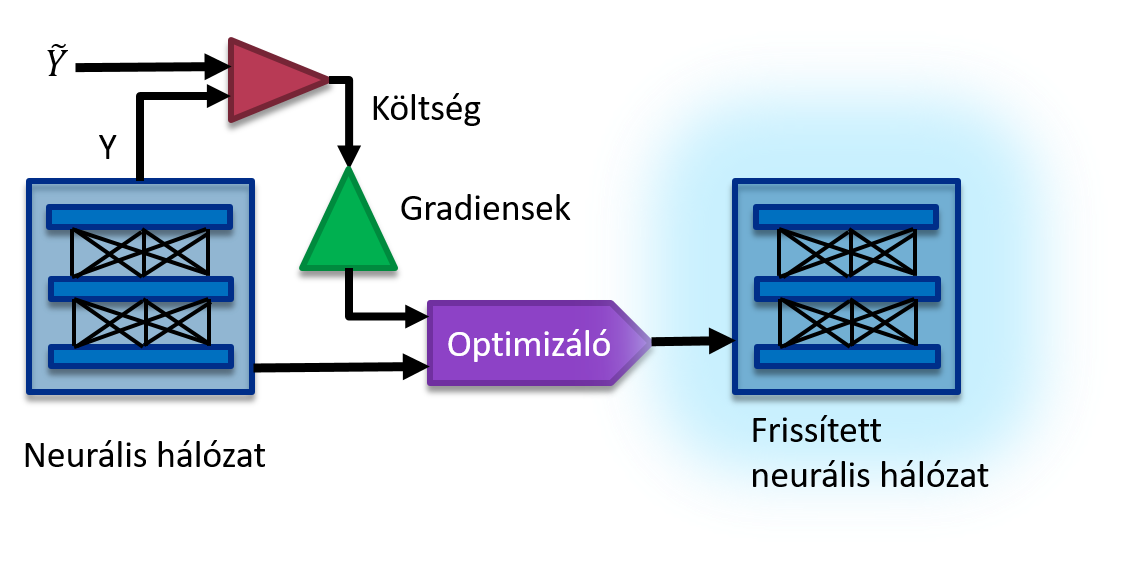
\includegraphics[width=100mm, keepaspectratio]{figures/nn-arch.png}
	\caption{Neurális hálózat architektúra.}
	\label{fig:nn-arch}
\end{figure}

Tegyük fel, hogy a \ref{fig:nn-arch} ábrán látható neurális hálózatot bináris klasszifikációra használjuk és hívjuk simán modellnek. A modell kezdeti paramétereit minden iterációban az optimizáló frissíti. A metatanítás az optimizációs algoritmus szempontjából azt jelenti, hogy az optimizáló állítható paramétereit nem mi állítjuk be kézzel, hanem a feladatot átadjuk egy másik modellnek, amit megtanítunk arra, hogy ezeket optimizálja miközben az eredeti modellünk tanul. Tehát az optimizáló az eredeti modellünk súlyait állítja, miközben a másik modellünk az optimizáló paramétereit javítja.

Ezzel absztrakciós szintet léptünk, ezt a másik modellt nevezzük metamodellnek. A metamodellnek ugyanúgy lesz meta-költségfüggvénye, meta-gradiensei és meta-optimizálója. Ugyanakkor látnunk kell, hogy ezt a metaoptimizálót is tekinthetjük modellnek és léphetünk feljebb metaszinteket, de előbb utóbb szükség lesz egy konkrét meta-optimizálóra, ami az alatta lévő optimizáló paramétereit állítja. 

\begin{figure}[!ht]
	\centering
	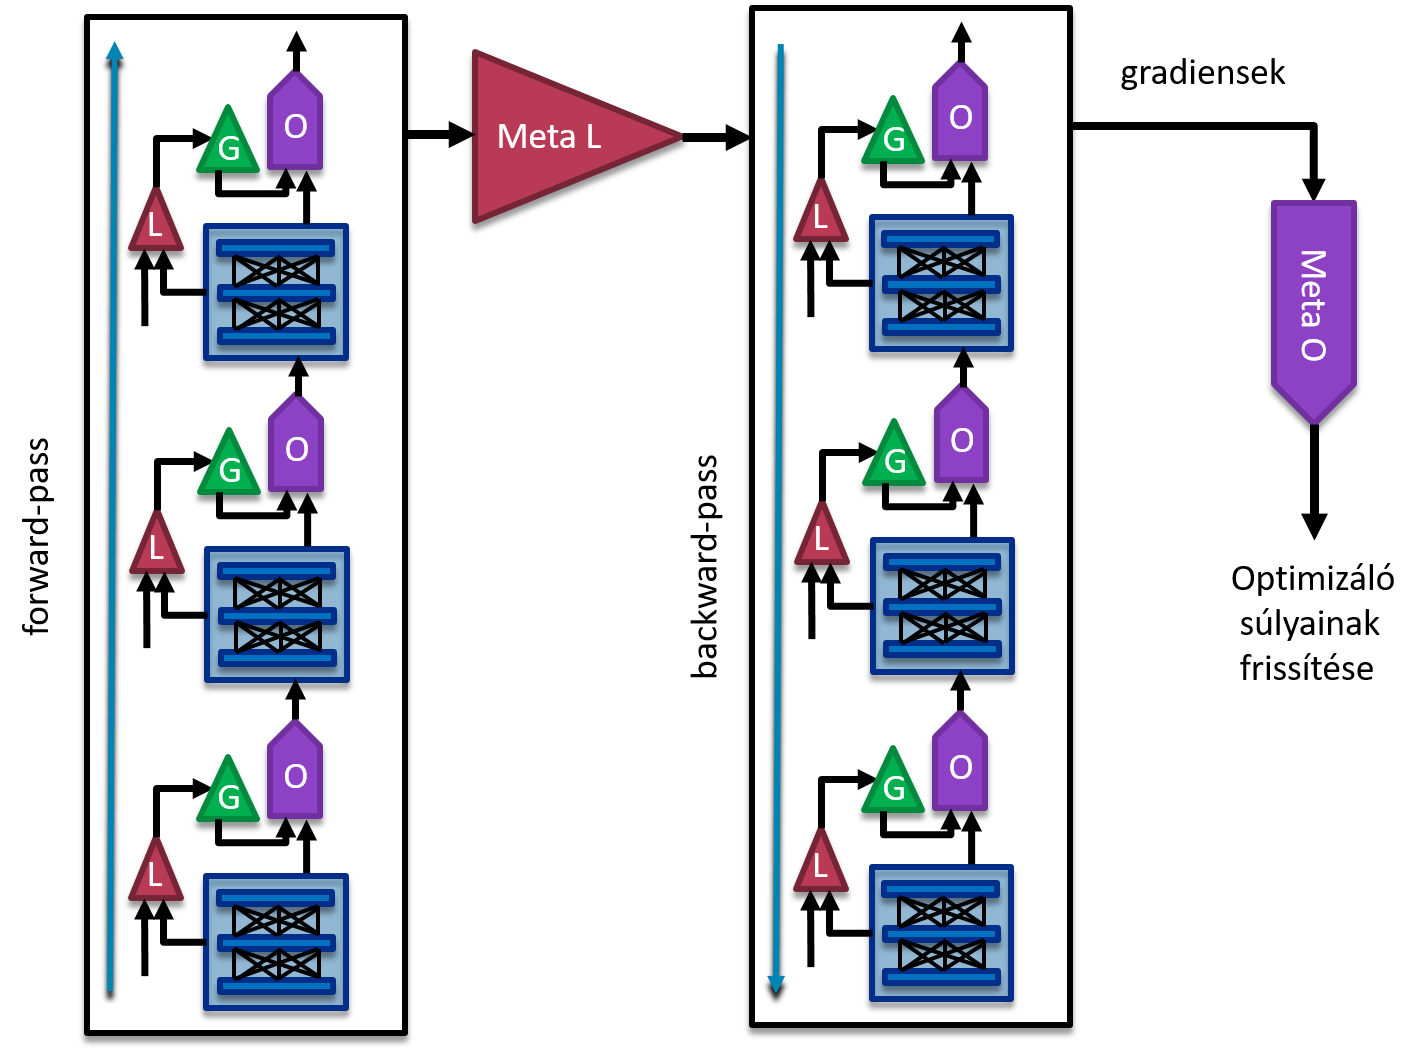
\includegraphics[width=120mm, keepaspectratio]{figures/meta-opt.png}
	\caption{Optimizáló metatanítás.}
	\label{fig:meta-opt}
\end{figure}

A \ref{fig:meta-opt} ábra az optimizáló metatanítást szemlélteti. A konkrét modell szinten  a fekete téglalapokban függőlegesen az eredeti bináris klasszifikációra használt modellünk tanítása történik, míg a téglalapok között vízszintesen a metamodell tanítása látszik.

A metaköltségnek vehetjük az eredeti modell költségeinek összegét egy adott iterációig. Ez jól leírja, hogy a modell tanul-e. A metaköltség-függvény alapján kiszámoljuk a meta-gradienseket, amit átadunk a metaoptimizálónak. Ez már egy konkrét optimizáló, például ADAM. Ezután a meta-optimizáló állítja az optimizáló paramétereit úgy, hogy csökkentse a meta-költséget, vagyis javítja a tanulási folyamatot. 

\subsection{Model-Agnostic Meta Learning (MAML)}


A MAML a modell kezdeti paramétereit optimalizálja úgy, hogy gyorsan tanuljon. Célja, hogy új, hasonló feladatokra kevesebb - akár egy - iterációval jó eredményt érjen el az optimizációs algoritmus. A modellt több feladathoz adaptálja a kezdeti paraméterei beállításával, így az kevés gradiens frissítés után képes megtanulni új feladatokat. Ez egy megközelítés a few-shot learning problémára.



\begin{figure}[!ht]
	\centering
	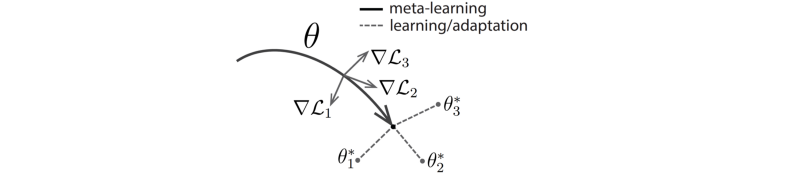
\includegraphics[width=200mm, keepaspectratio]{figures/maml.png}
	\caption{A MAML algoritmus vizualizációja. (Finn et al 2017)}
	\label{fig:maml}
\end{figure}

Legyen a modell egy $f_\theta$ függvény, ahol $\theta$ jelöli a modell paramétereit. Amikor a modellt egy új $\mathcal{T}_i$ feladathoz adaptáljuk, a modell $\theta$ paramétereit változtatjuk $\theta'_i$-re. Az adaptált paraméter egy gradiens frissítés esetén a következő:

\begin{equation} \label{eq:1}
\theta'_i = \theta - \alpha\nabla_{\theta}\mathcal{L}_{\mathcal{T}_i}(f_{\theta})
\end{equation}

A \ref{fig:maml} ábrán a $\theta$ jelöli a modell kezdeti súlyait. A szürke vonalak a $\nabla\mathcal{L}_1$, $\nabla\mathcal{L}_2$, $\nabla\mathcal{L}_3$ gradienseket
mutatják, a $\theta^*_1$, $\theta^*_2$, $\theta^*_3$ pedig az adott feladathoz adaptált modell optimális paraméterei. A vastag vonal a metatanulási folyamatot mutatja. Látható, hogy a $\theta$ paraméterű modell jelenlegi helyzetében közel van mindhárom feladat optimális paramétereihez, tehát kevés gradiens frissítéssel finomhangolható bármelyikre.

\begin{algorithm}
	\caption{Model-Agnostic Meta Learning}
	\label{fig:maml-pseudo}
	\begin{algorithmic}[1]
		\Require $p(\mathcal{T})$: distribution over tasks
		\Require $\alpha$, $\beta$ step size hyperpatameters
		\State randomly initialize $\theta$
		\While{not done}
		\State Sample batch of tasks $\mathcal{T}_i \sim p(\mathcal{T})$
		\ForAll{$\mathcal{T}_i$}
		\State Evaluate $\nabla_{\theta}\mathcal{L}_{\mathcal{T}_i}(f_{\theta})$ with respect to K examples
		\State Compute adapted parameters with gradient descent: $\theta'_i = \theta - \alpha\nabla_{\theta}\mathcal{L}_{\mathcal{T}_i}(f_{\theta})$
		\EndFor
		\State Update $\theta \gets \theta - \beta\nabla_{\theta}\sum_{\mathcal{T}_i\sim p(\mathcal{T})}\mathcal{L}_{\mathcal{T}_i} (f_{\theta'_i})$
		\EndWhile
	\end{algorithmic}
\end{algorithm}

Az algoritmus először veszi a $\mathcal{T}$ feladatok egy $p(\mathcal{T})$ eloszlását és a modell kezdeti paramétereit véletlen módon inicializálja. A feladatok közül kiválaszt párat és mindegyikre $K$ tanítómintával tanítja a modellt. A tanítás során gradiens frissítésekkel kiszámolja az optimális $\theta_i$ modellparamétereket \ref{eq:1} szerint. 
A meta-célfüggvényt az adaptált $\theta_i$ paraméterekkel kiszámolt költségek összege adja a $\mathcal{T}_i$ feladatokon.

\begin{equation} \label{eq:2}
\min_\theta \sum_{\mathcal{T}_i\sim p(\mathcal{T})}\mathcal{L}_{\mathcal{T}_i}(f_{\theta'_i})=
\sum_{\mathcal{T}_i\sim p(\mathcal{T})}\mathcal{L}_{\mathcal{T}_i}(f_{\theta-\alpha\nabla_{\theta}\mathcal{L}_{\mathcal{T}_i}(f_{\theta})})
\end{equation}
 
Mielőtt új $\mathcal{T_i}$ feladatokat választ, sztochasztikus gradient descent módszerrel frissíti a modell kezdeti paramétereit a meta-célfüggvény szerint.
 
\subsection{Reptile}

A reptile algoritmus nagyon hasonlít a MAML-hoz. Ugyanúgy a hálózat kezdeti súlyait incicializálja úgy, hogy további hasonló feladatokra könnyen általánosítható legyen. A MAML-hoz képest előnye, hogy kevesebb számítást igényel, nincs szükség második deriváltak kiszámolására, csak SGD-t futtat a feladatokon.


\begin{algorithm}
	\caption{Reptile}
	\label{fig:reptile-pseudo}
	\begin{algorithmic}[1]
		\State Initialize $\phi$, the vector of initial parameters
		\For{iteration = 1, 2, $\dots$}
		\State Sample task $\tau$, corresponding to loss $L_{\tau}$ on weight vectors $\tilde\phi$
		\State Compute $\tilde\phi = U^k_{\tau}(\phi)$, denoting $k$ steps of SGD or Adam
		\State Update $\phi \gets \phi + \epsilon(\tilde\phi - \phi)$
		\EndFor
	\end{algorithmic}
\end{algorithm}

Adott a szigma kezdeti paraméter vektor. Valamennyi iteráción keresztül választunk egy véletlen feladatot és futtatjuk rajta valahányszor az SGD algoritmust, ami a $\phi$ paraméter vektorból a $\tilde\phi$-t eredményezi. Ezután javítjuk a modell kezdeti paramétereit a megadott szabály szerint.

\section{Modell alapú metatanítás}

A modell alapú metatanítás lényege az olyan modelleket tervezése, amelyek képesek kevés tanítással, gyorsan javítani a paramétereiket. Egy ismert implementáció a Memory-Augmented Neural Networks, ami neurális Turing-gépeket használ.
